\problemname{}
\newcommand\name{Brianna}


\name{} is a bookworm. At home, she has a big bookshelf with all her favourite
books. She has a large collection ranging from detective novels and
science-fiction novels to biographies.

Recently, \name{} has expanded her collection with $n$ graphic novels. However,
the new books currently lie around everywhere and form huge stacks on the floor.
In the meantime, one of the shelf boards has collected dust and random household utensils that
do not belong there.
The new books just lying around have become too much to bear,
and \name{} finally decided to put them
on this shelf board. To do so, she first has to make room on it.

\begin{figure}[!h]
	\centering
	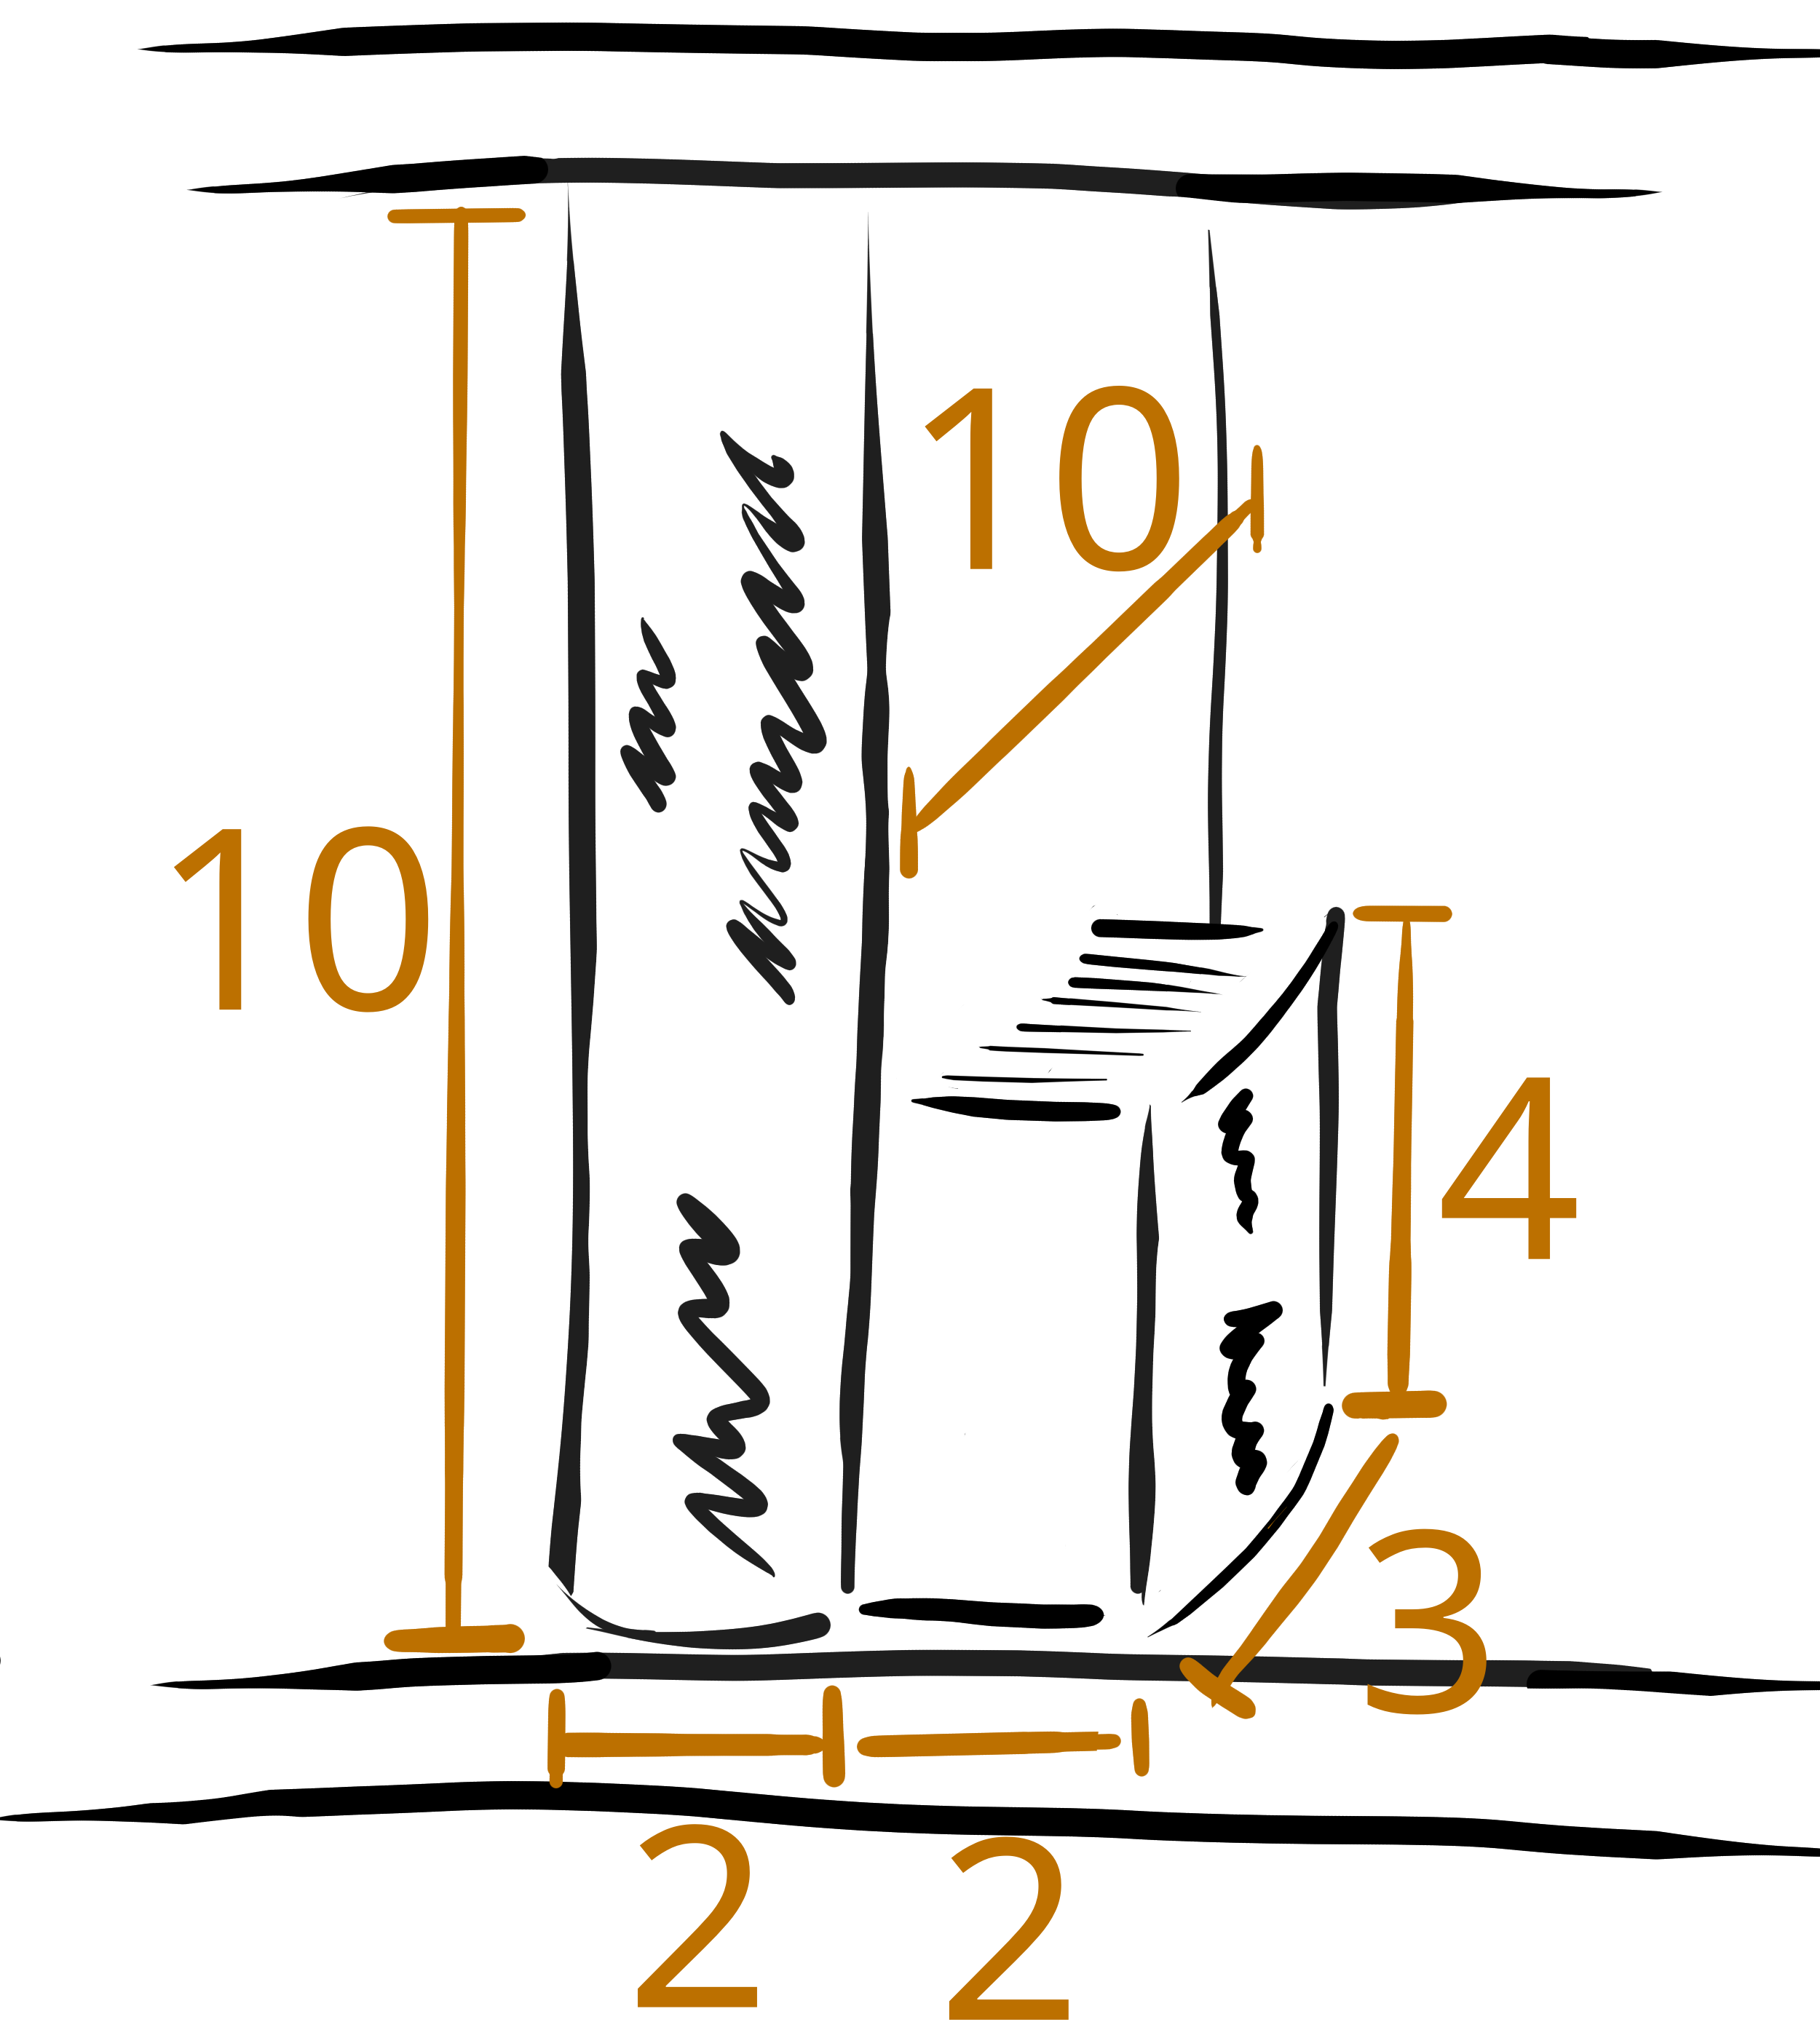
\includegraphics[width=0.25\textwidth]{books}
	\caption{Visualization of Sample Input 3.}
\end{figure}

\name{} wants to arrange the books in a single horizontal line without
stacking multiple books on top of each other. While the shelf is wide
enough to hold all books without problems, it takes time to make room 
on the shelf. Therefore, \name{} wants to minimize the width of the part 
of the shelf that she needs to clear.

Each book can be described as a cuboid with three side lengths $l$, $w$, and $h$.
Since the room above the shelf board is limited by the next shelf board above it,
she can only fit a book vertically if its vertical side length is at most the distance $H$
between the two shelf boards. \name{} may rotate each book
in three-dimensional space as she wants. It is guaranteed that the shelf is deep enough
so that the books will not fall off, no matter the orientation. However, all books must
stand properly on the shelf board, meaning that every book touches the shelf board along an
entire face and not just by an edge.

What is the minimum width of shelf \name{}'s books need?

\begin{Input}
    The input consists of:
    \begin{itemize}
        \item One line with two integers $n$ and $H$ ($1\leq n\leq 10^5$, $1\leq H \leq 10^9$), the number of books and the height of the shelf, respectively.
        \item $n$ lines, each containing three integers $l$, $w$, $h$ ($1\leq l,w,h \leq 10^9$), the dimensions of the books.
    \end{itemize}
\end{Input}

\begin{Output}
    Output the minimum width of shelf \name{}'s books need, or ``\texttt{impossible}'' if it is impossible to place the books on the shelf.
\end{Output}
